\section{Non-Relativistic Mass Distribution}
\label{sec_classical}
\begin{quotation}
	\raggedleft \it I know that this defies the law of gravity, \\ but, you see, I never studied law. \\ -- Bugs Bunny
\end{quotation}
In order to obtain the mass distribution of the fermion ball, let us first look at a simple Newtonian model 
\cite{ref_classicalapproach}, in which the gravitational potential satisfies Poisson's equation
\begin{equation}
	\nabla \Phi(r) = -4 \pi G \rho_{\nu}(r)
	\label{eqn_poisson}
\end{equation}
where $G$ is Newton's gravitational constant and $\rho_{\nu}(r)$ the mass density of the fermions and anti-fermions at a
particular radius $r$. The self-gravity of the fermionic matter may be balanced with its degeneracy pressure, obeying the
equation of hydrostatic equilibrium
\begin{equation}
	\frac{1}{\rho_{\nu}} \frac{dP_{\nu}}{dr} + \frac{d\Phi}{dr} = 0
	\label{eqn_hydroequil}
\end{equation}
Here the pressure is given by the polytropic equation of state for non-relativistic fermionic matter at zero temperature.
\begin{equation}
	P_{\nu} = K \rho_{\nu}^{\frac{5}{3}}
	\label{eqn_polytropic}
\end{equation}
with the constant $K$ given by \cite{ref_thomasfermiapproach}
\begin{equation}
	K = \left(\frac{6}{g_{\nu}}\right)^{\frac{2}{3}} \frac{\pi^{\frac{4}{3}} \hbar^2}{5 m_{\nu}^{\frac{8}{3}}}
	\label{eqn_polytropicconstant}
\end{equation}
where $g_{\nu}$ represents the number of degrees of freedom of the fermions (spin and particle-antiparticle degeneracy),
either 2 (Majorana) or 4 (Dirac), $m_{\nu}$ being the fermion rest mass. We thus obtain
\begin{equation}
	\frac{5}{2} K \rho^{\frac{2}{3}} + \Phi = E_0
	\label{eqn_classicalarb1}
\end{equation}
with $E_0$ as the potential at the outer radius ($R_0$). Taking the fermion ball to be spherically symmetric
(and hence the gravitational potential), it follows from (\ref{eqn_poisson}) that
\begin{equation}
	\frac{1}{r}\frac{d^2(r\Phi)}{dr^2} = -4 \pi G \rho_{\nu}(r)
	\label{eqn_classicalarb2}
\end{equation}
and using the substitution
\begin{equation}
	f = E_0 - \Phi = \frac{5}{2} K \rho^{\frac{2}{3}}
	\label{eqn_classicalarb3}
\end{equation}
the Poisson equation may be re-written as
\begin{equation}
	\frac{1}{r}\frac{d^2(rf)}{dr^2} = -4 \pi G \left(\frac{2f}{5K}\right)^{\frac{3}{2}}
	\label{eqn_classicalarb4}
\end{equation}
By defining $u = rf$, (\ref{eqn_classicalarb4}) is more easily solved. It is now more convenient to work in the dimensionless
units as given by
\begin{eqnarray}
	&&v = \frac{u}{GM_\odot}
	\label{eqn_classicalv} \\
	&&x = \frac{r}{a_\nu}
	\label{eqn_classicalx}
\end{eqnarray}
with
\begin{equation}
	a_{\nu} = \frac{5K}{2G M_\odot^\frac{1}{3} (4\pi)^\frac{2}{3}}
	\label{eqn_classicalanu}
\end{equation}
\subsection{Lan\'e-Emden Equation}
The previous substitutions reduce (\ref{eqn_classicalarb4}) to the Lan\'e-Emden equation
\begin{equation}
	\frac{d^2v(x)}{dx^2} = -\frac{v(x)^\frac{3}{2}}{x^\frac{1}{2}}
	\label{eqn_laneemden}
\end{equation}
which must be solved numerically. The boundary conditions are set such that $u$ disappears at the outer radius $R_0$ (where the
fermion density is zero) and the enclosed mass tends to $M_B$ at the origin of the fermion ball. $M_B$ is an arbitrary central
baryonic mass, resident at the centre, allowing for the placement of a possible 'small' black hole or compact star cluster
($M_{\nu \overline{\nu}}$ the corresponding total fermionic mass). This implies
\begin{eqnarray*}
	v(0) = \frac{M_B}{M_\odot} \qquad
	v(x_0) = 0
\end{eqnarray*}
\begin{figure}[!htb]
	\begin{center}
	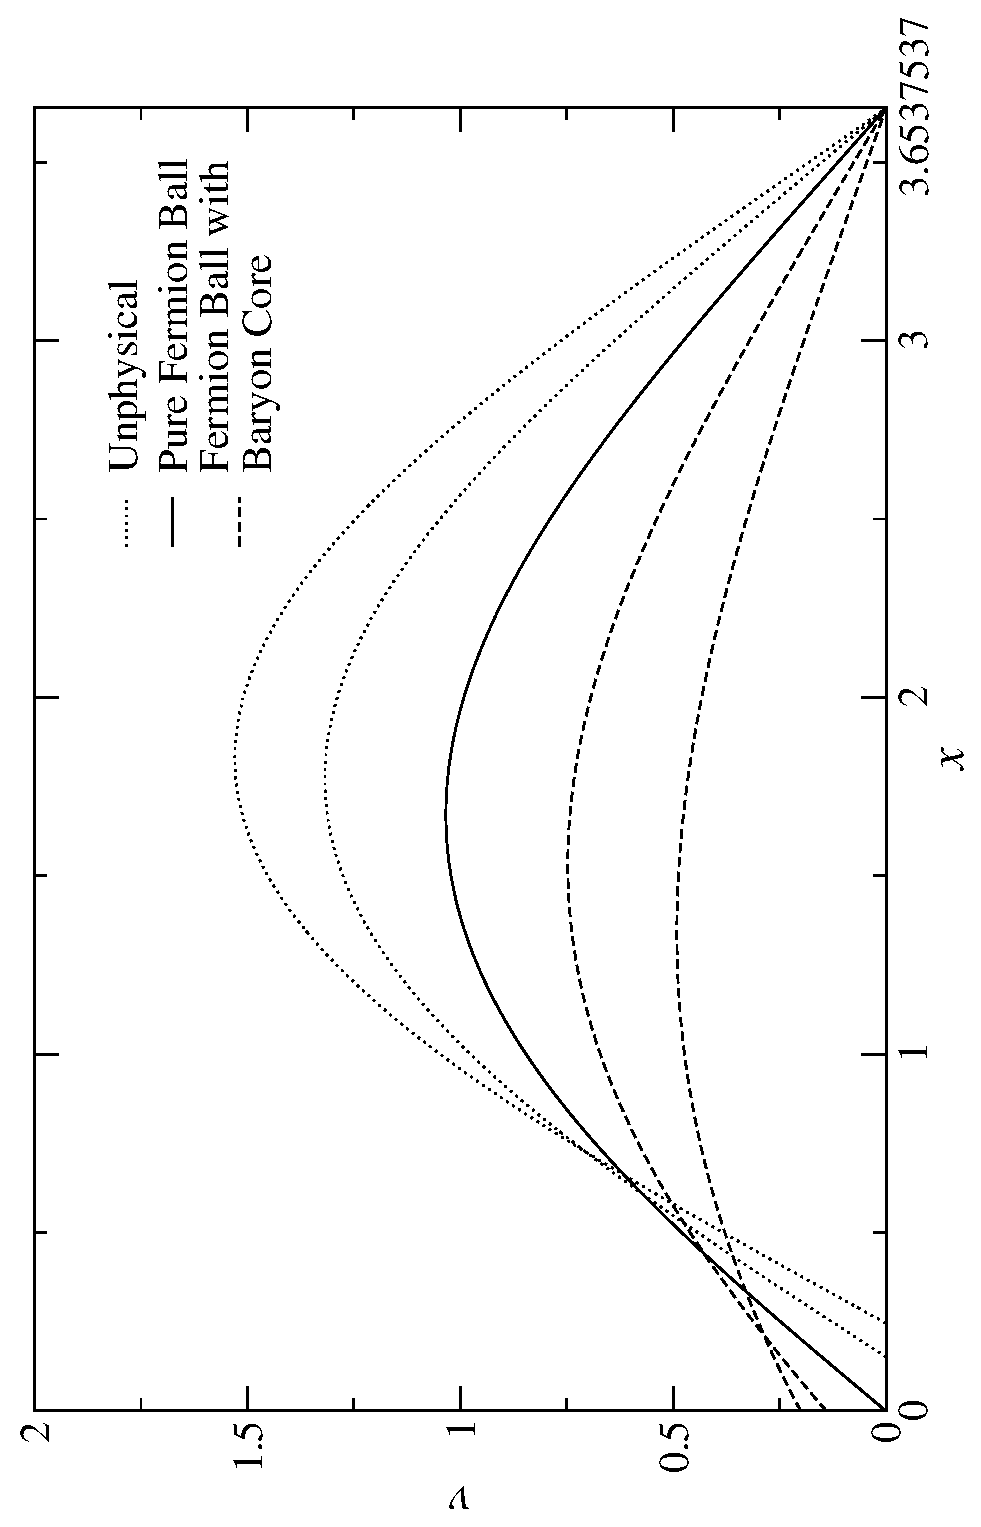
\includegraphics[angle=-90,width=0.9\textwidth]{eps/laneemden.eps}
	\caption{Solutions of the Lan\'e-Emden equation}
	\label{fig_laneemden}
	\end{center}
\end{figure}
The enclosed mass is found at any radius by integrating over the density
\begin{equation}
	M(r) = \int^r_0 4 \pi \rho_\nu (r) r^2 dr
	\label{eqn_classicalmassintegral}
\end{equation}
resulting for any dimensionless radius $x$ as
\begin{equation}
	M(x) = M_\odot\left[v(x)-xv'(x)\right]
	\label{eqn_classicalmass}
\end{equation}
and from (\ref{eqn_classicalarb3}), the gravitational potential is given as
\begin{equation}
	\Phi(x) = \frac{G M_\odot}{a_\nu}\left[v'(x_0)-\frac{v(x)}{x}\right]
	\label{eqn_classicalpotential}
\end{equation}
By the homology theorem, if $v(x)$ is a solution of the Lan\'e-Emden equation, then
\begin{equation}
	\widetilde v(\widetilde x) = A^3 v(Ax)
	\label{eqn_classicalhomology}
\end{equation}
is also a solution, as long as $A$ is a positive real number. This has several implications on the other quantities, and they must
be scaled accordingly. Radii, enclosed mass and gravitational potential scale as
\begin{eqnarray*}
	\widetilde R_0 = \frac{R_0}{A} \qquad
	\widetilde M(\widetilde x) = A^3 M(x) \qquad
	\widetilde \Phi = A^4 \Phi(x)
\end{eqnarray*}
It is then sensible to solve the Lan\'e-Emden equation only once and scale this to the required mass of the fermion ball.
In the numerical solution, an initial value is required for $v'$, whether we choose to solve outward from the origin, or
inward from the outer radius. This is initially set (arbitrarily) to unity, and by solving outward the endpoint value
$x_0$ is obtained, allowing the equation to be solved inward with any $v'(x_0)$, corresponding to a central baryonic
mass given by (before scaling) 
\begin{equation}
	\frac{dv(x_0)}{dx} = - \frac{M_B+M_{\nu \overline{\nu}}}{x_0M_\odot}
	\label{eqn_classicalinitialdvdr}
\end{equation}
Several solutions are shown in Figure \ref{fig_laneemden}.
Using these solutions for $v(x)$ and $v'(x)$, it is now possible with the aid of (\ref{eqn_classicalmass}) and
(\ref{eqn_classicalpotential}) to calculate the mass distribution and potential within the fermion ball. Enclosed mass solutions are
shown in Figure \ref{fig_classicalmassdist}, potentials in Figure \ref{fig_classicalpotential}.

Although in these calculations we have allowed for a baryonic object at the centre, there is no direct evidence to suggest that this
may be the case. A baryonic object must have a
very large mass in order to make a significant impact on the overall mass distribution, for this reason, all further calculations will
assume that $M_B$ is zero, and we therefore have a pure fermion ball.
\begin{figure}[p]
	\begin{center}
	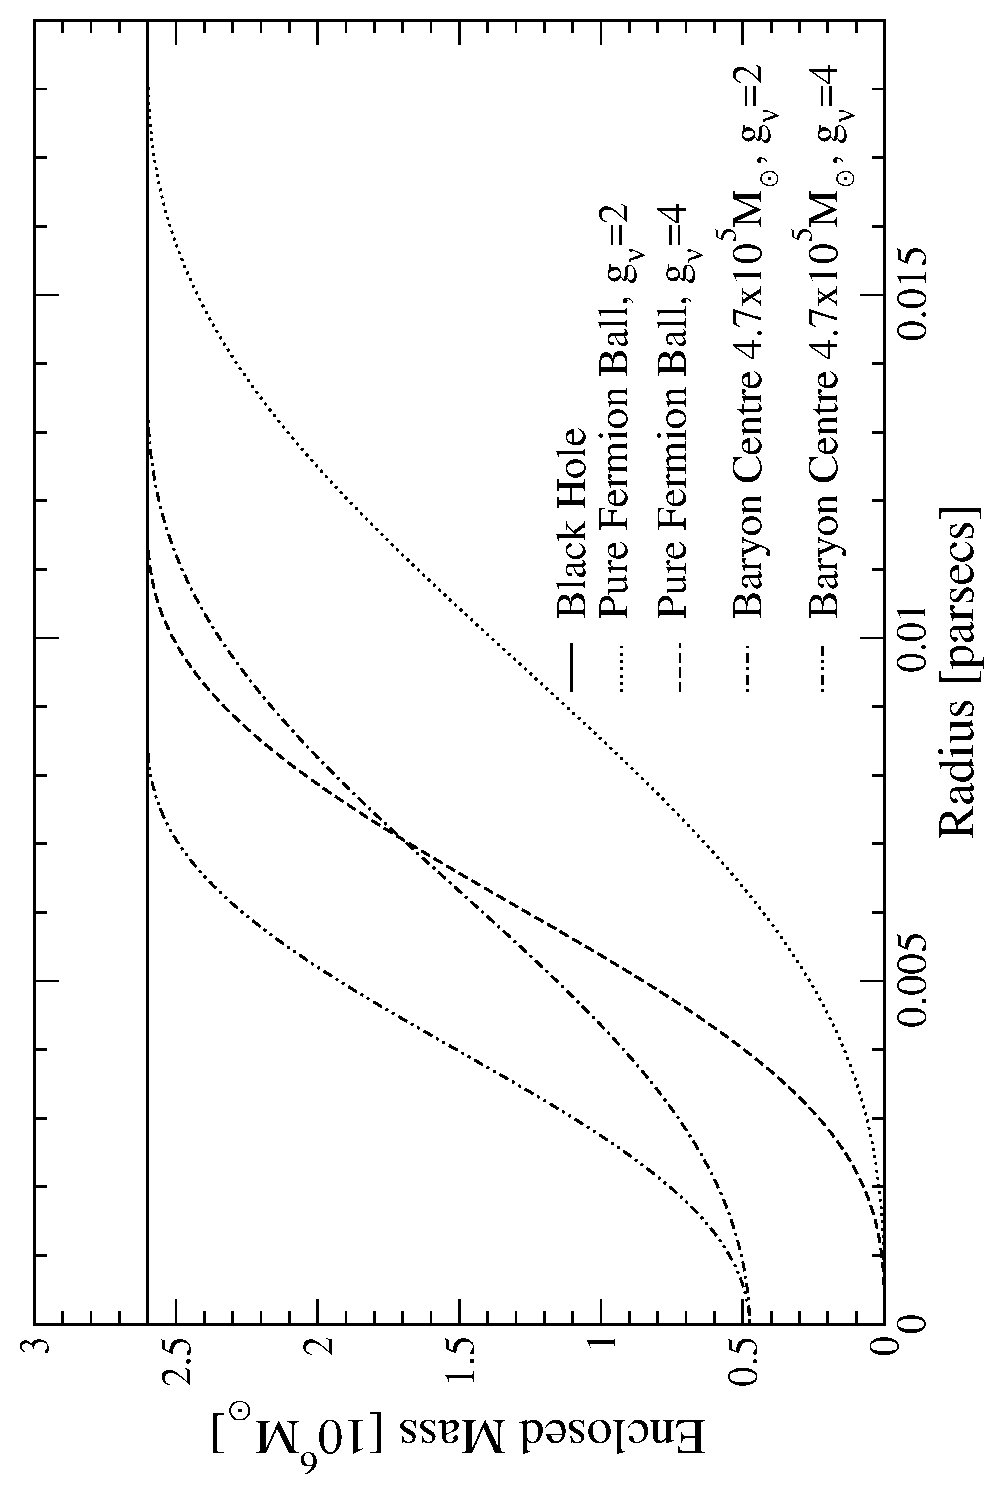
\includegraphics[angle=-90,width=0.9\textwidth]{eps/classicalmassdist.eps}
	\caption{Enclosed mass distribution as a function of radius for 16keV fermions. The solid line denotes a black hole,
	which exhibits a constant enclosed mass at all radii.}
	\label{fig_classicalmassdist}
	\end{center}
\end{figure}
\begin{figure}[p]
	\begin{center}
	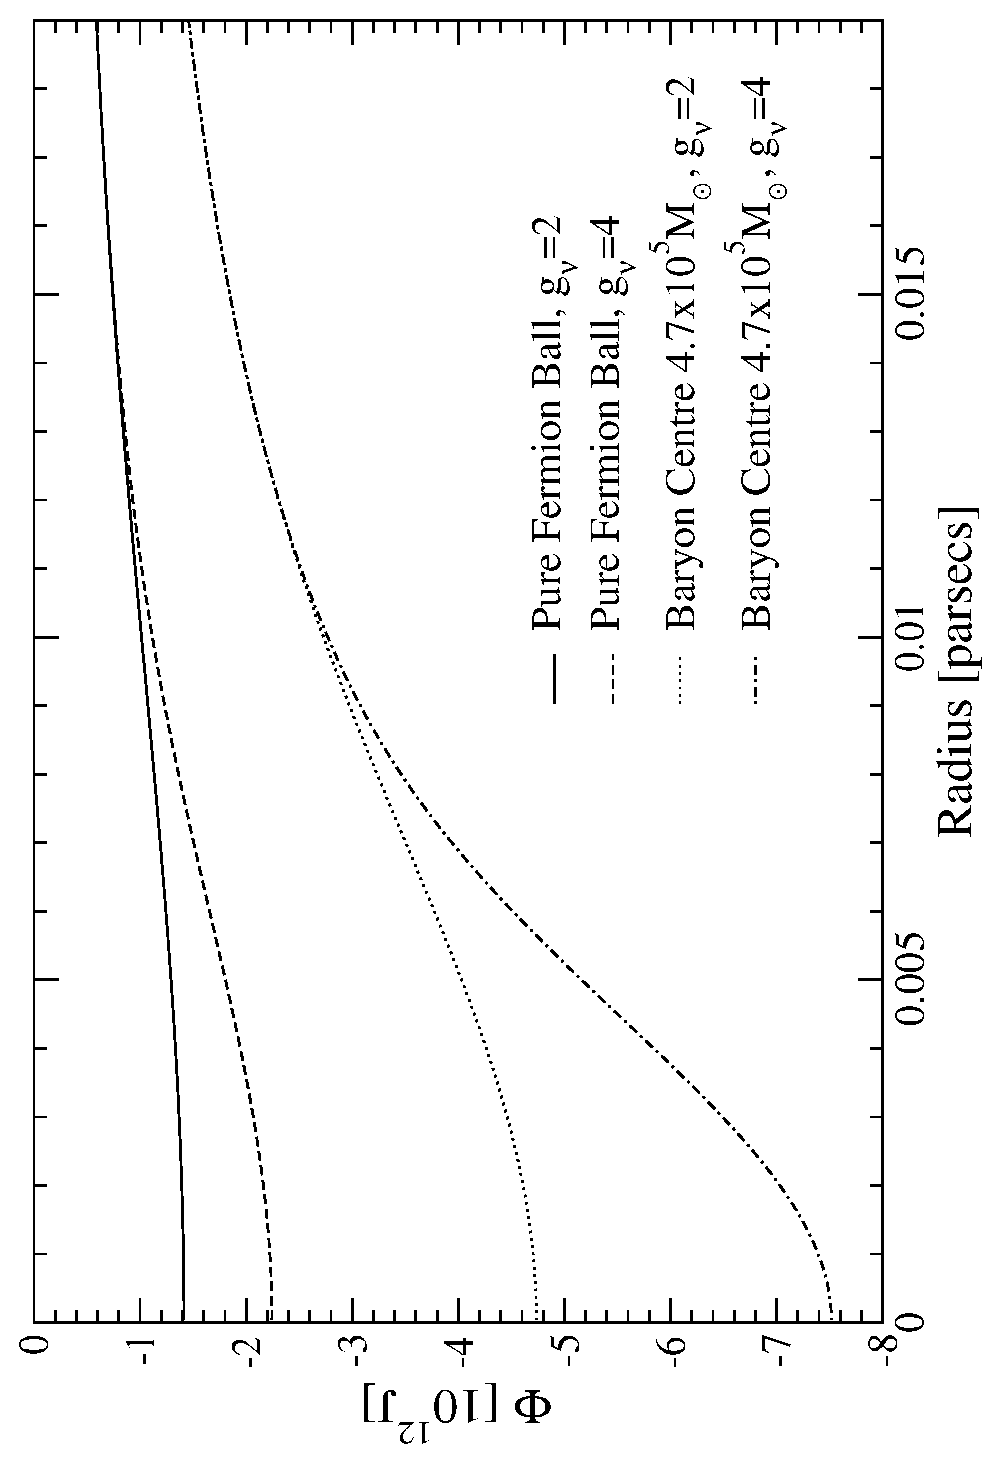
\includegraphics[angle=-90,width=0.9\textwidth]{eps/classicalpotential.eps}
	\caption{Gravitational potential as a function of radius for 16keV fermions.}
	\label{fig_classicalpotential}
	\end{center}
\end{figure}
\subsubsection{Thomas-Fermi}
The Newtonian mass distribution can also be described using the statistical method due to Thomas and Fermi
\cite{ref_thomasfermi}, in which the local Fermi energy is set to the local gravitational binding energy \cite{ref_thomasfermiapproach}.
The Lan\'e-Emden equation (\ref{eqn_laneemden}) has much in common with the Thomas-Fermi equation, containing only an extra negation. The
fermions are gravitationally attractive, opposed to electro-statically repulsive as in atomic physics where the Thomas-Fermi equation is
applied. It is interesting to note that in 1928 Majorana found a semi-analytical solution to the Thomas-Fermi equation which remained
unpublished until 2001 \cite{ref_majoranasolution}, unfortunately the method cannot be directly applied to the Lan\'e-Emden equation.

\subsection{Limits on Fermion Mass}
\label{sec_fermionlimits}
Although these solutions are for 16keV fermions, solutions are easily obtainable for a variety of fermion masses. However, the overall
fermion ball radius and mass is dependent upon the individual rest mass of the fermions and their degeneracy. As such, the minimal
$m_\nu$ in order to constrain the ball fully within the boundaries of a total mass ($M_T$) and a maximal radius ($R_0$) is given by
\begin{equation}
	m_\nu \ge \left( \frac{ - 3 x_0^4 v'(x_0) \pi^2 \hbar^6}{64} \right)^\frac{1}{8} \left(\frac{1}{M_T R_0^3 g_\nu^2}\right)^\frac{1}{8}
	\label{eqn_classicalfermionmass}
\end{equation}

Proper motion analysis \cite{ref_ghezmotion} has imposed an enclosed mass of $2.6 \pm 0.2 \times 10^6 M_\odot$ at a radius of 0.015pc.
Figure \ref{fig_classicalfermionmass} displays several possible mass distributions corresponding to fermion rest masses. It is clear
that when experimental errors are accounted for, the minimal allowed $m_\nu$ is approximately 16keV. For this reason, all calculations
from here on in will be performed using 16keV fermions. This is based on the assumption that the fermion ball is fully constrained
within the 0.015pc, a more massive fermion ball with fermions of lesser $m_\nu$ would still reproduce the results of
\cite{ref_ghezmotion}, and this may be important later.
\begin{figure}[!tb]
	\begin{center}
	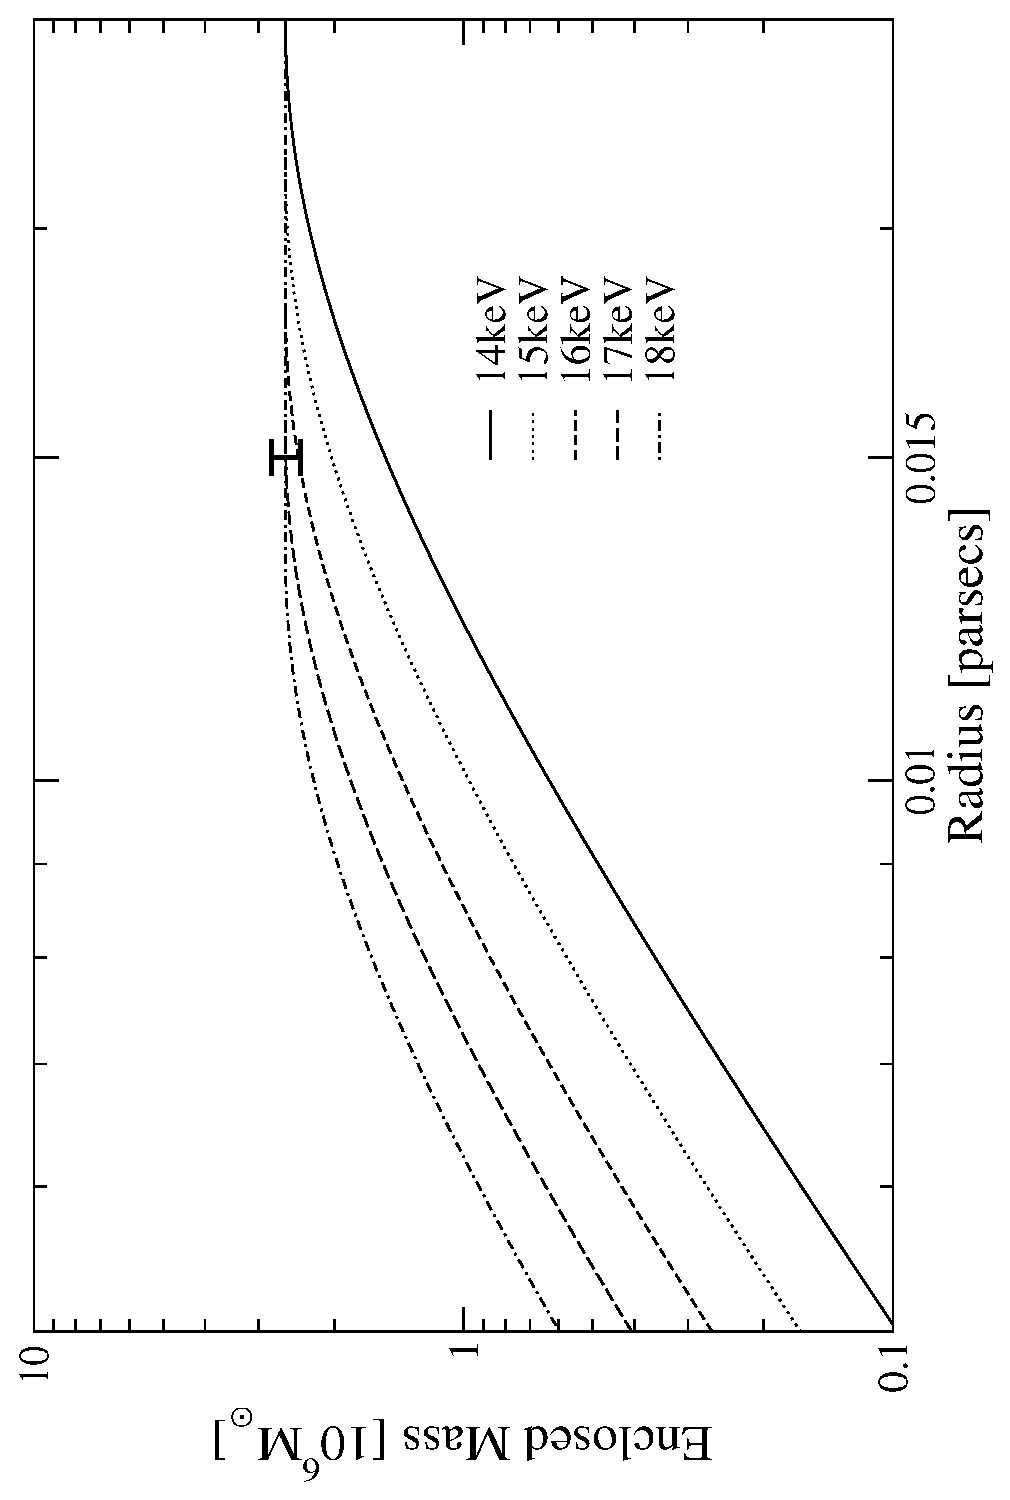
\includegraphics[angle=-90,width=0.9\textwidth]{eps/classicalfermionmass.eps}
	\caption{The enclosed mass as a function of radius for various fermion masses. Data point is from \cite{ref_ghezmotion}.}
	\label{fig_classicalfermionmass}
	\end{center}
\end{figure}
It is also worth noting that the mass distribution for $g_\nu=2$ fermions can easily be reproduced for $g_\nu=4$ by slightly
decreasing the rest mass according to
\begin{equation}
	m_\nu g_\nu^{\frac{1}{4}} = \overline{m}_\nu \overline{g}_\nu^{\frac{1}{4}}
	\label{eqn_classicalfermiondegeneracyrelation}
\end{equation}
